\section*{Appendix}
\appendix

\begin{comment}
Appendix: Put all Figures, Tables, Algorithms, etc., in appendix.

\section{First Appendix}
\label{app:FirstAppendix}

\begin{figure}[tbh]

\includegraphics[width=.45\textwidth]{Images/sdu-logo.png}
\caption{SDU Logo}
\label{app:fig:SDULogo}
\end{figure}

\section{Second Appendix}
\label{app:SecondAppendix}

\begin{figure*}[tbh]

\includegraphics[width=.95\textwidth]{Images/sdu-logo.png}
\caption{Full width figure SDU Logo}
\label{app:fig:SDULogoV2}
\end{figure*}
\end{comment}


\section{UPPAAL Models}
\label{app:UPPAALModels}

TODO: Add UPPAAL models here

\section{Validation Tests}
\label{app:ValidationTests}

TODO: Add validation tests here

\section{Wiring Diagram}
\label{app:WiringDiagram}

\begin{figure}[tbh]
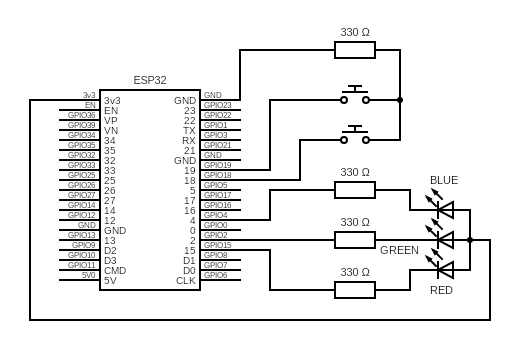
\includegraphics[width=.95\textwidth]{./../circuit/circuit.png}
\caption{Hardware wiring diagram}
\label{app:fig:WiringDiagram}
\end{figure}

\section{LED Colors}
\label{app:LEDColors}
None - unlocked and closed
\newline
Green - locked and closed
\newline
red - unlocked and open
\newline
yellow - locked and open
\newline
yellow/white - locked, open and alarm
\newline
green/cyan - locked, closed and alarm
\newline
! purple - unlocked, open and alarm
\newline
! blue - alarm
\newline
! are states that does not exist in the UPPAAL models.